\begin{frame}{CCSD $\op{T}_2$ amplitude equation - Derivation }
    \note{Filename: ccsd\_diagramderivation03.tex}

    \begin{equation*}
        0 = \bra{\Phi_{ij}^{ab}} \barh \ket{\Phi_0}
    \end{equation*}
    \begin{columns}
    \column{0.5\textwidth}
    \begin{itemize}
        \item Two pairs of particle/hole  external lines.
        \item Final excitation level: +2
    \end{itemize}
    \column{0.5\textwidth}
    \begin{figure}
        \centering
        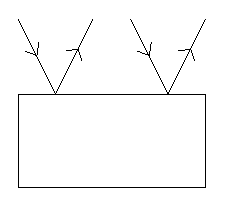
\includegraphics[scale=0.45]{graphics/t2amp_diag}
    \end{figure}
    \end{columns}
    \renewcommand{\figurename}{Elements}
    \begin{columns}[t]
    \column{0.75\textwidth}
    \begin{figure}
        \caption{$\op{H}_N$}
        \centering
        \parbox{0.20\textwidth}{
            \centering
            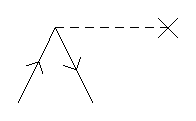
\includegraphics[scale=0.35]{graphics/f1}} 
        \parbox{0.20\textwidth}{
            \centering
            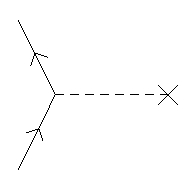
\includegraphics[scale=0.35]{graphics/f2}} 
        \parbox{0.20\textwidth}{
            \centering
            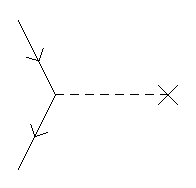
\includegraphics[scale=0.35]{graphics/f3}} 
        \parbox{0.20\textwidth}{
            \centering
            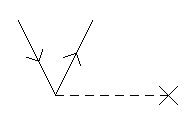
\includegraphics[scale=0.35]{graphics/f4}} 
        \parbox{0.20\textwidth}{
            \centering
            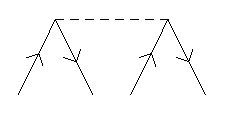
\includegraphics[scale=0.35]{graphics/v1}} 
        \parbox{0.20\textwidth}{
            \centering
            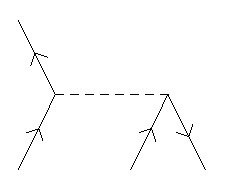
\includegraphics[scale=0.35]{graphics/v2}} 
        \parbox{0.20\textwidth}{
            \centering
            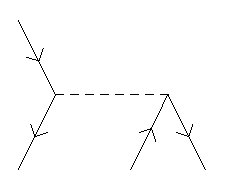
\includegraphics[scale=0.35]{graphics/v3}} 
        \parbox{0.20\textwidth}{
            \centering
            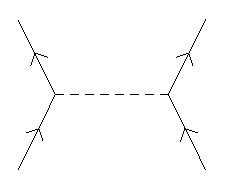
\includegraphics[scale=0.35]{graphics/v4}} 
        \parbox{0.20\textwidth}{
            \centering
            
\includegraphics[scale=0.35]{graphics/v5}} 
        \parbox{0.20\textwidth}{
            \centering
            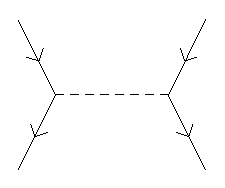
\includegraphics[scale=0.35]{graphics/v6}} 
        \parbox{0.20\textwidth}{
            \centering
            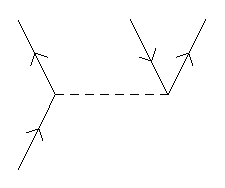
\includegraphics[scale=0.35]{graphics/v7}} 
        \parbox{0.20\textwidth}{
            \centering
            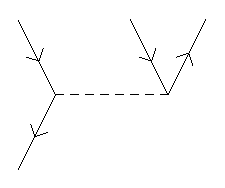
\includegraphics[scale=0.35]{graphics/v8}} 
        \parbox{0.20\textwidth}{
            \centering
            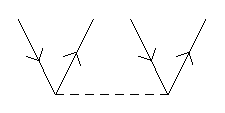
\includegraphics[scale=0.35]{graphics/v9}} 
    \end{figure}
    \column{0.25\textwidth}
    \begin{figure}
        \caption{$\op{T}$}
        \centering
        \parbox[height=3cm]{0.60\textwidth}{
            \centering
            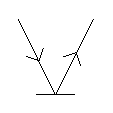
\includegraphics[scale=0.45]{graphics/t1}} 
    \end{figure}
    \begin{figure}
        \parbox[height=3cm]{0.60\textwidth}{
            \centering
            
\includegraphics[scale=0.45]{graphics/t2}} 
    \end{figure}
\end{columns}


\end{frame}

    
